\subsection{Demonstration der Visualisierung am Anwedungsbeispiel}

Die Anwendung des Prototyps wird nachfolgend demonstriert, wobei die visuelle Übersichtlichkeit, die farbliche Informationskodierung und die interaktive Handhabung im Vordergrund stehen. In der Benutzeroberfläche des Systems, wie sie in Abbildung ? dargestellt ist, 

nachfolgend anhand der Testgebiete in der \textit{Gohliser Straße} sowie im \textit{Mariannenpark} demonstriert,wobei die visuelle Übersichtlichkeit, die farbliche Informationskodierung und die interaktive Handhabung im Vordergrund stehen. In der GUI werden die 3D-Punktwolken des gewählten Abschnitts über ein DOP gelegt, um realen Umgebungsverhältnissen zu demonstrieren und die Orientierung zu erleichtern.


\begin{figure}[htbp]
    \centering
    \newcommand{\bildhoehe}{4.0cm}
    
        \begin{subfigure}[b]{0.49\textwidth}
        \centering
        \includegraphics[height=\bildhoehe, width=\textwidth, keepaspectratio]{imgs/vis/Straße-nach-ID.png}
        \caption{Straßen nach Segment-ID}
    \end{subfigure}
    \hfill
    \begin{subfigure}[b]{0.49\textwidth}
        \centering
        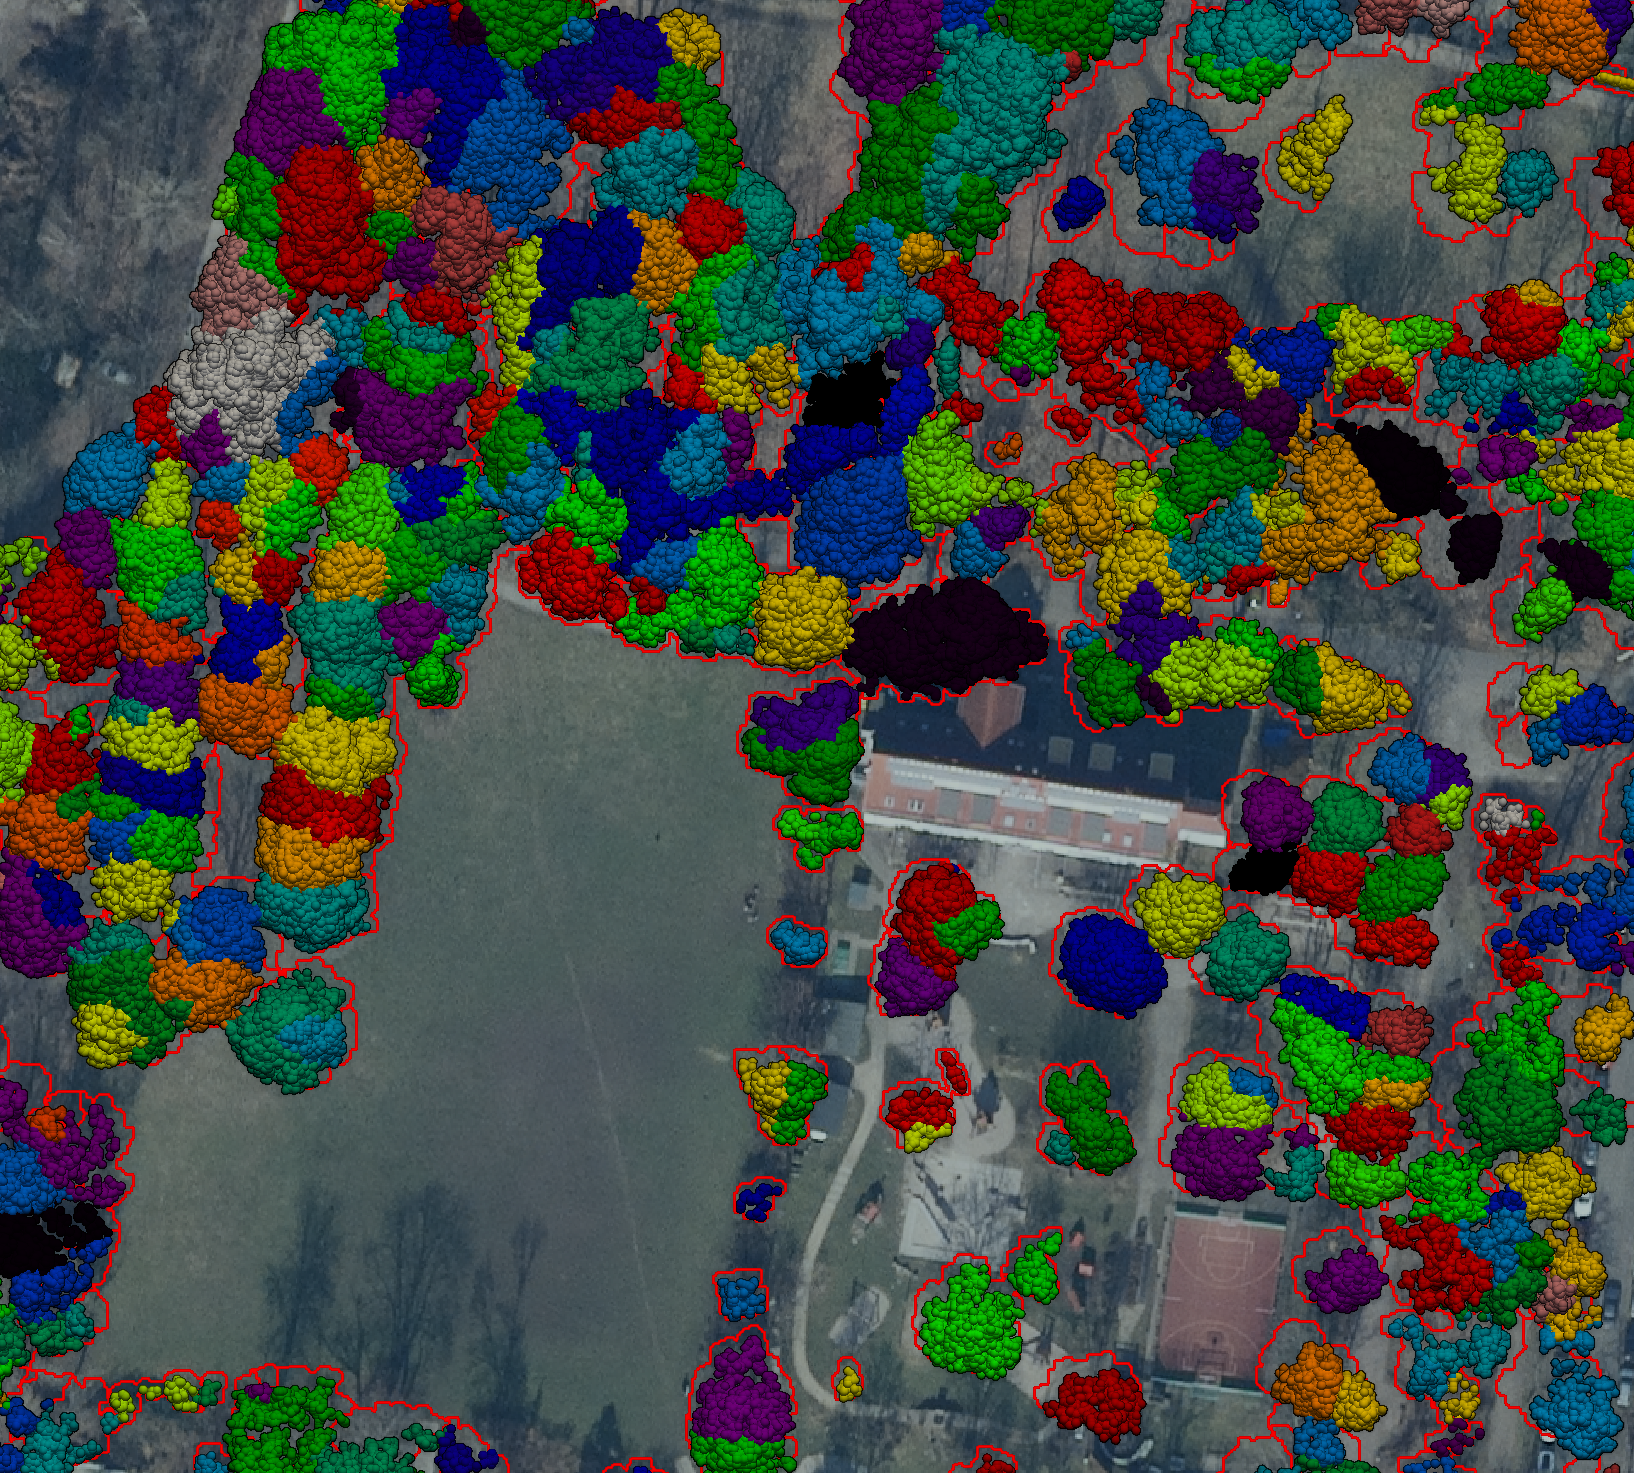
\includegraphics[height=\bildhoehe, width=\textwidth, keepaspectratio]{imgs/vis/Park-nach-ID.png}
        \caption{Park nach Segment-ID}
    \end{subfigure}

    % Zeile 1
    \begin{subfigure}[b]{0.49\textwidth}
        \centering
        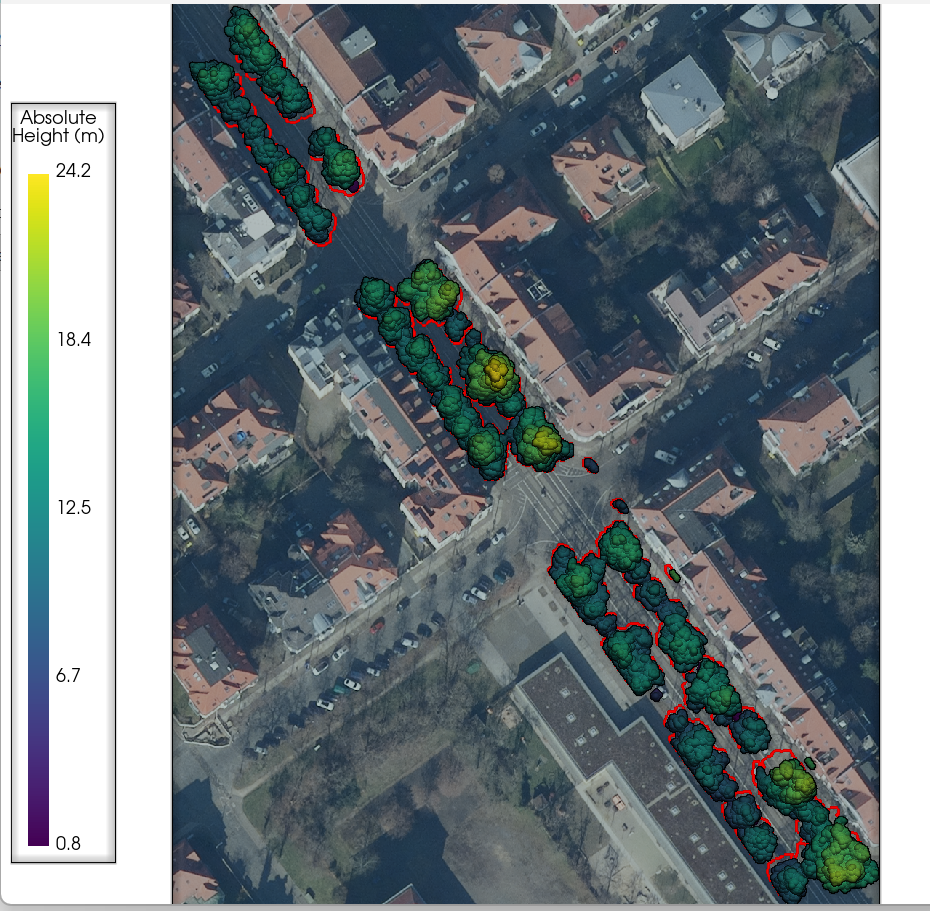
\includegraphics[height=\bildhoehe, width=\textwidth, keepaspectratio]{imgs/vis/Straße-nach-abs-hoehe.png}
        \caption{Straßen: abs. Höhe}
    \end{subfigure}
    \hfill
    \begin{subfigure}[b]{0.49\textwidth}
        \centering
        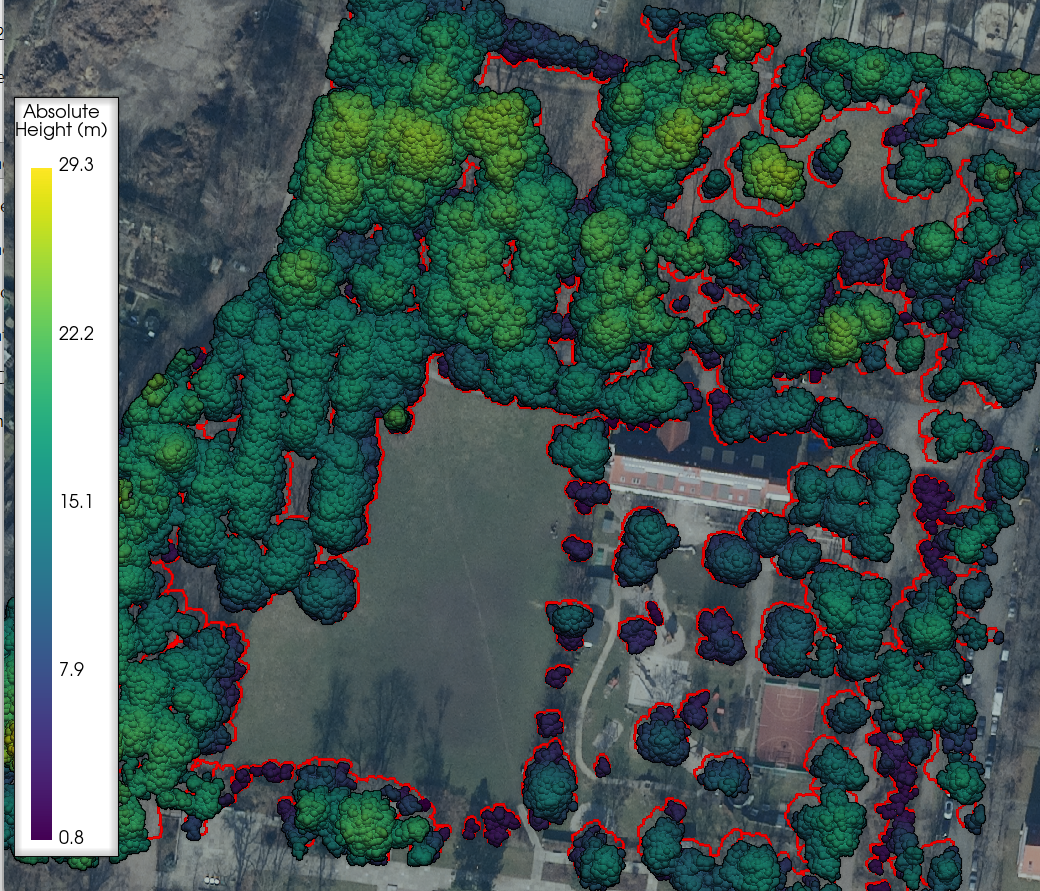
\includegraphics[height=\bildhoehe, width=\textwidth, keepaspectratio]{imgs/vis/Park-nach-abs-hoehe.png}
        \caption{Park: abs. Höhe}
    \end{subfigure}

    \vspace{0.3cm}
    % Zeile 2
    \begin{subfigure}[b]{0.49\textwidth}
        \centering
        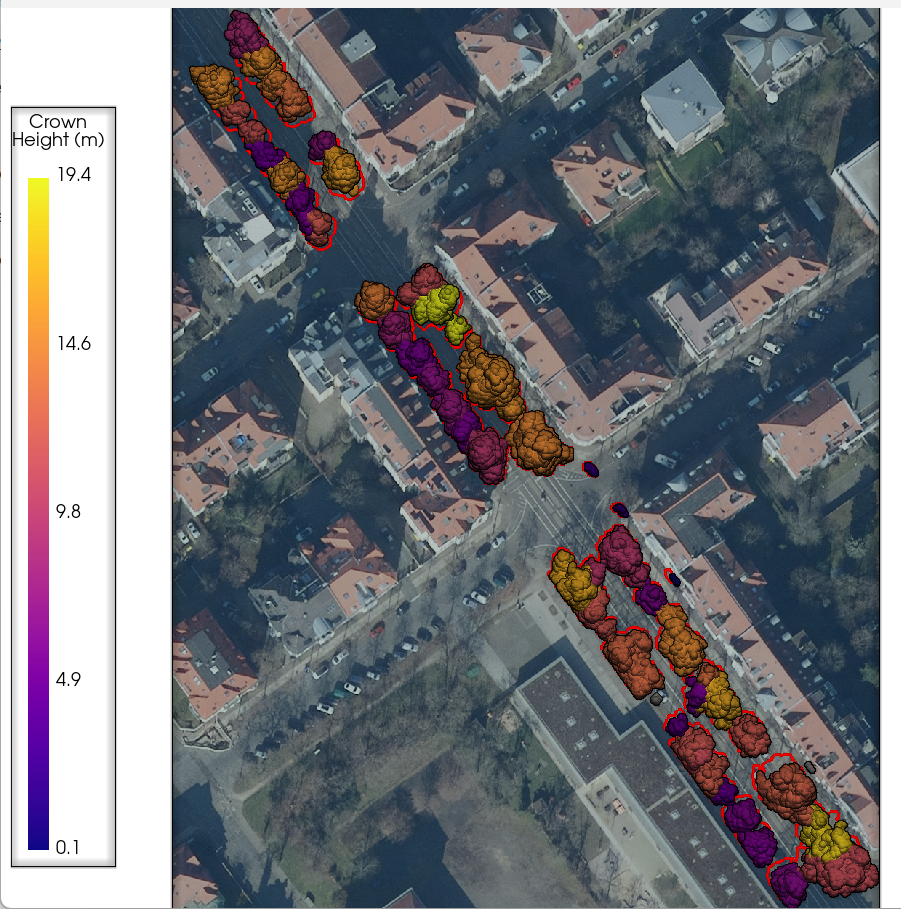
\includegraphics[height=\bildhoehe, width=\textwidth, keepaspectratio]{imgs/vis/Straße-nach-Kronenhoehe.png}
        \caption{Straßen: Kronenhöhe}
    \end{subfigure}
    \hfill
    \begin{subfigure}[b]{0.49\textwidth}
        \centering
        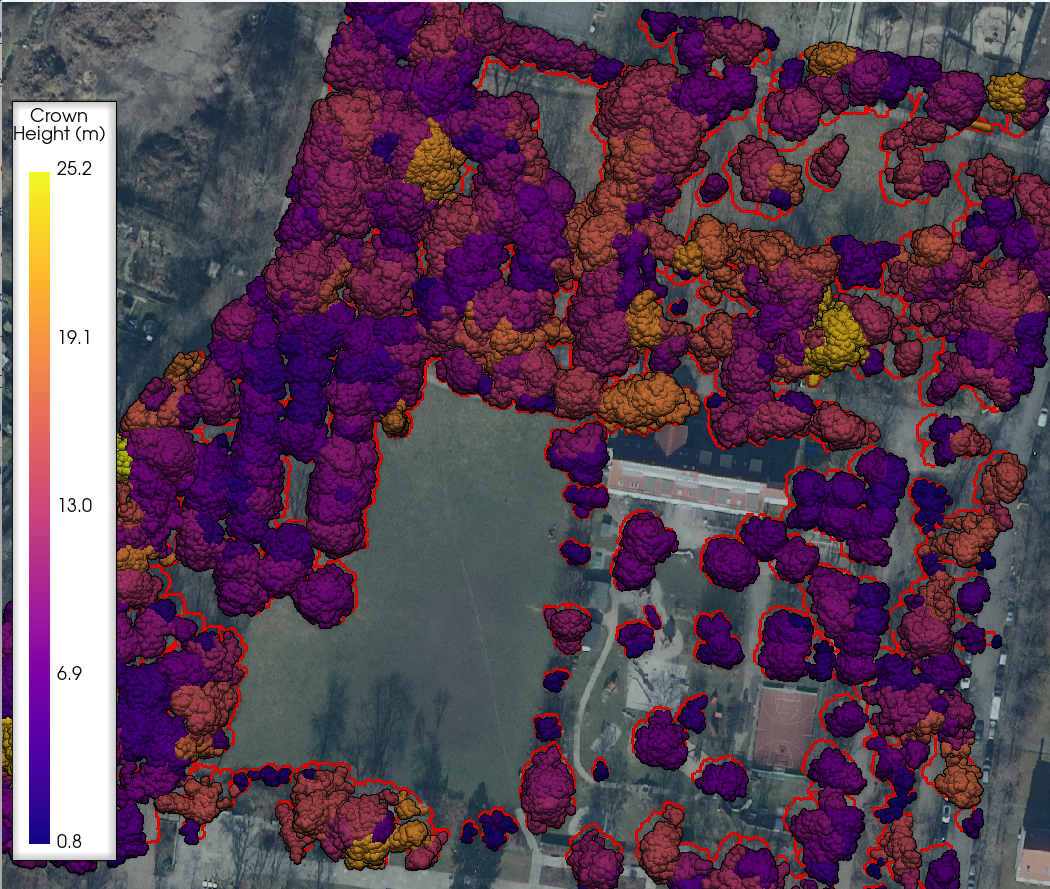
\includegraphics[height=\bildhoehe, width=\textwidth, keepaspectratio]{imgs/vis/Park-nach-Kronenhoehe.png}
        \caption{Park: Kronenhöhe}
    \end{subfigure}

    \vspace{0.3cm}
    % Zeile 3
    \begin{subfigure}[b]{0.49\textwidth}
        \centering
        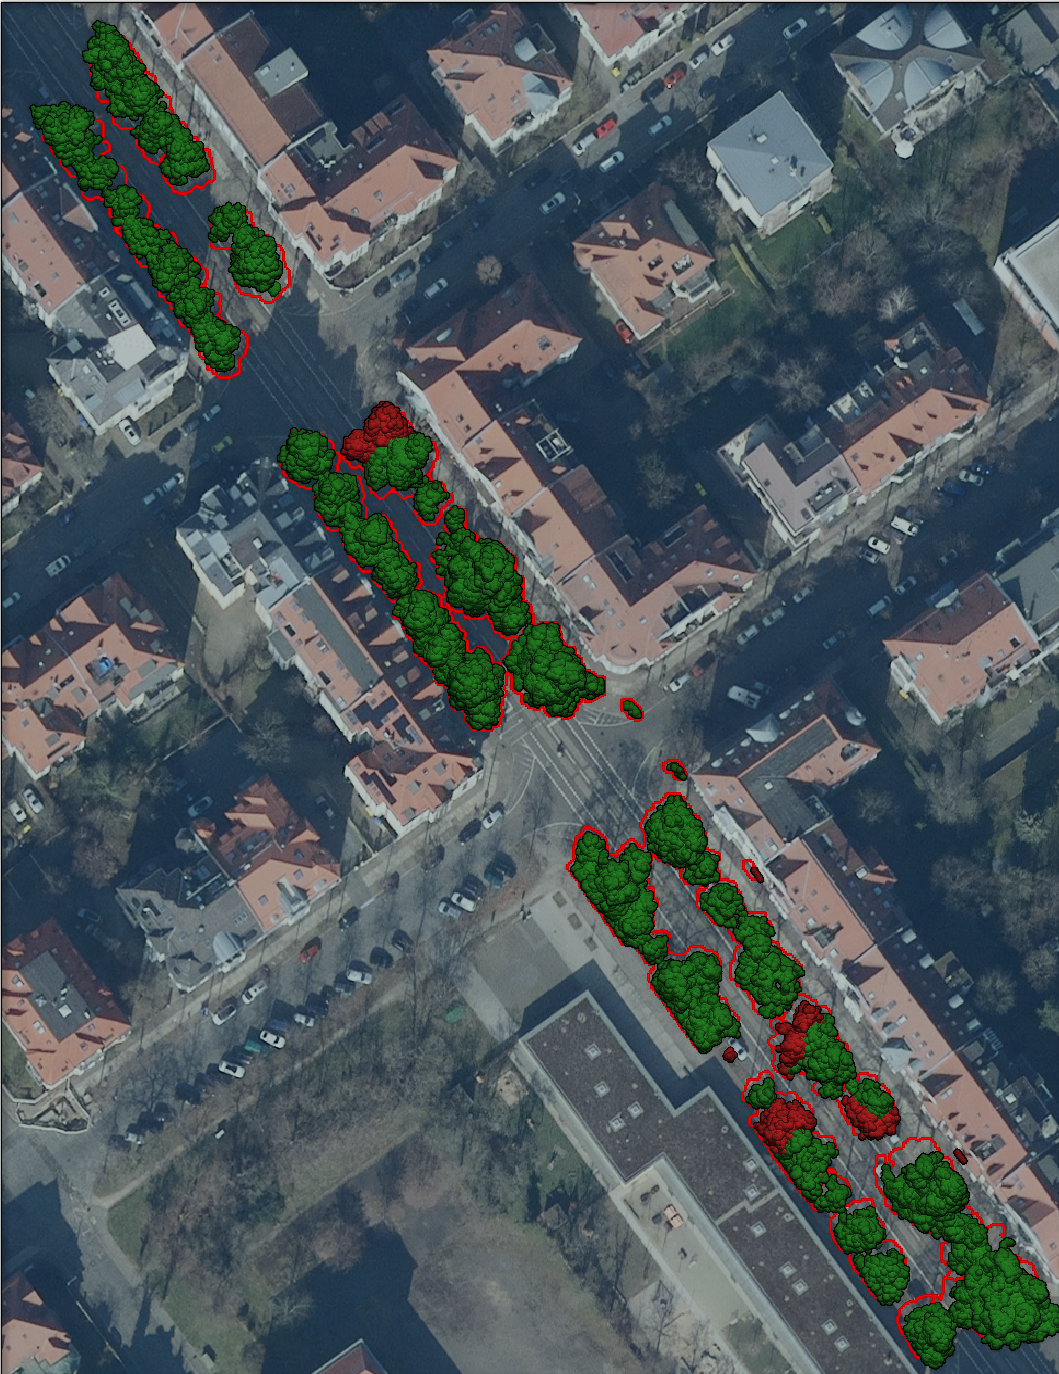
\includegraphics[height=\bildhoehe, width=\textwidth, keepaspectratio]{imgs/vis/Straße-Katastermatch.png}
        \caption{Straßen: Kataster-Match}
    \end{subfigure}
    \hfill
    \begin{subfigure}[b]{0.49\textwidth}
        \centering
        \includegraphics[height=\bildhoehe, width=\textwidth, keepaspectratio]{imgs/vis/Park-Katastermatch.png}
        \caption{Park: Kataster-Match}
    \end{subfigure}

    \vspace{0.3cm}
    % Zeile 4
    \begin{subfigure}[b]{0.49\textwidth}
        \centering
        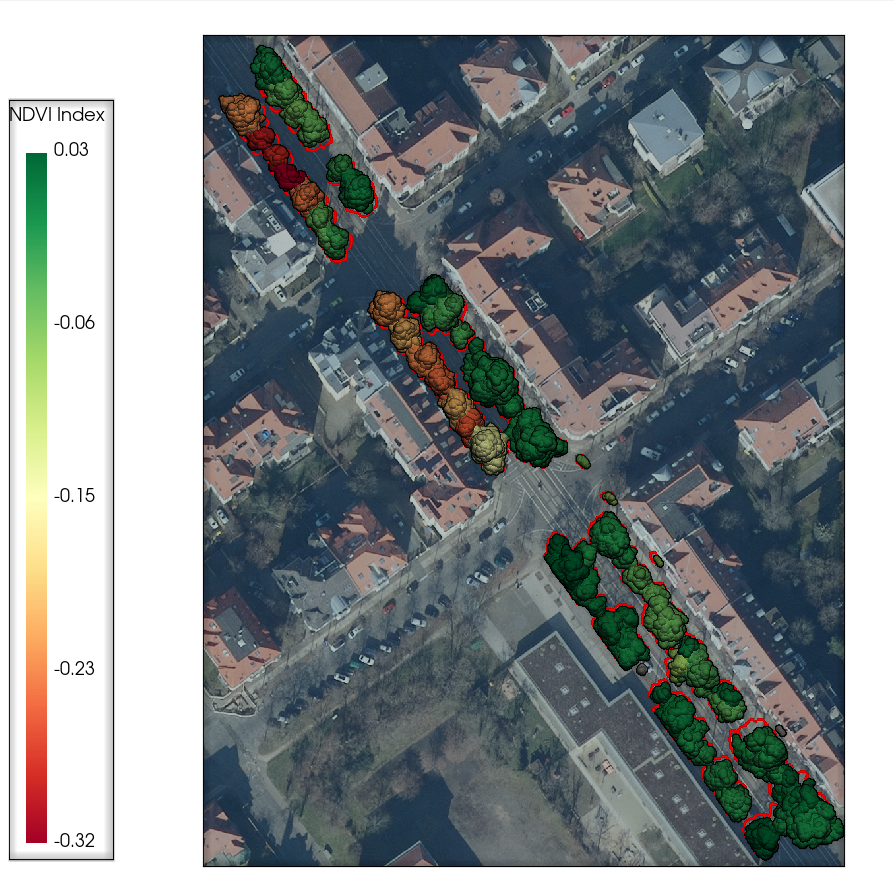
\includegraphics[height=\bildhoehe, width=\textwidth, keepaspectratio]{imgs/vis/Straße-NDVI.png}
        \caption{Straßen: mittlerer NDVI}
    \end{subfigure}
    \hfill
    \begin{subfigure}[b]{0.49\textwidth}
        \centering
        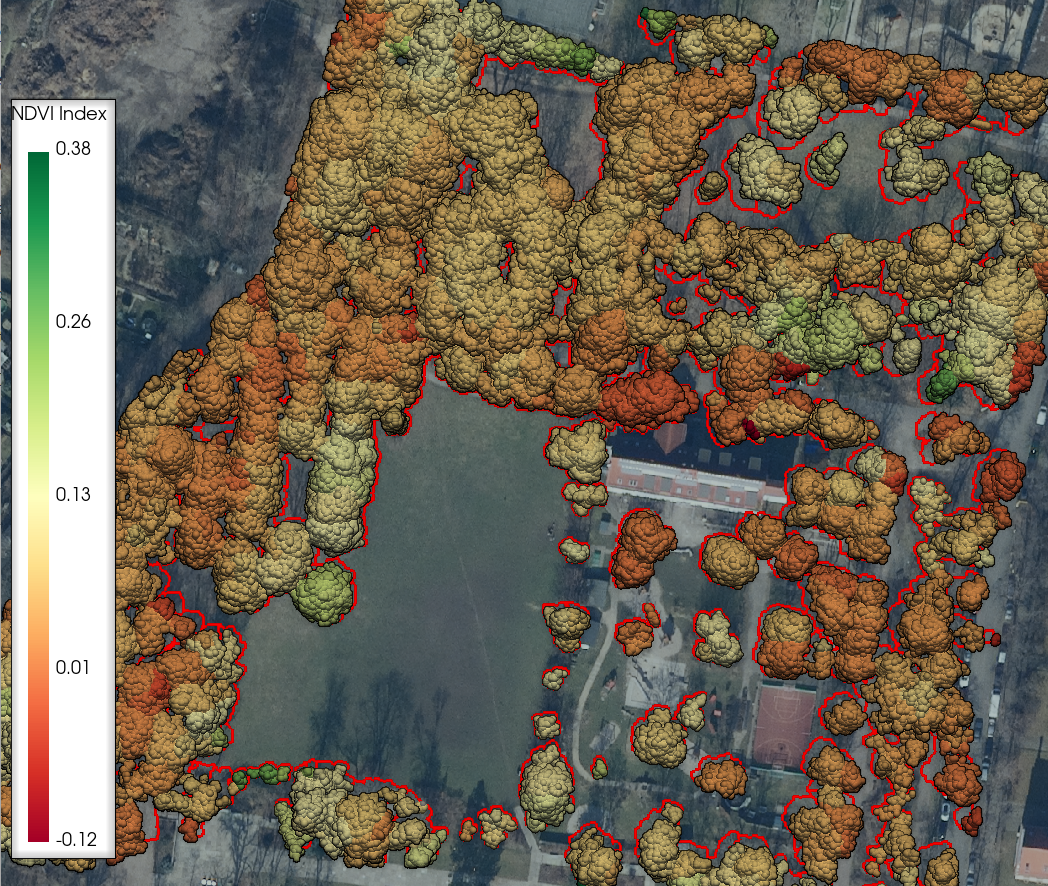
\includegraphics[height=\bildhoehe, width=\textwidth, keepaspectratio]{imgs/vis/Park-NDVI.png}
        \caption{Park: mittlerer NDVI}
    \end{subfigure}
    \caption{Einfärbungen der Punkte nach verschiedenen Parametern jeweils für Straßen- und Parkbäume}
    \label{fig:vis-coloring-grid}
\end{figure}

Die Funktionen verschiedener Einfärbungsmodi machen geometrische, physiologische und administrative Attribute der Bäume direkt sichtbar. Die Standarddarstellung nach Segment-ID ermöglicht besonders für das dichte Kronendach in Parks (Abbildung \ref{fig:park-ID}), eine klare visuelle Trennung eng zusammenstehenden Bäume. Beim Wechsel auf die absolute Höhe werden die strukturellen Unterschiede zwischen den Gebieten deutlich. Die Straßenbäume weisen mit einer maximalen Höhe von 24,2 m ein homogenes Höhenniveau auf, wohingegen der Mariannenpark eine ausgeprägte vertikale Staffelung zeigt und in den dichten Kronenbereichen Spitzenhöhen von bis zu 29,3 m erreicht. Ein analoges Bild liefert die reine Kronenhöhe, die im Straßenraum bei kompakteren Kronen maximal 19,4 m beträgt, im vielschichtigen Parkbestand jedoch Werte von bis zu 25,2 m erreicht.

Diese geometrische Analyse wird durch die physiologischen und administrativen Visualisierungsmodi fachlich ergänzt. Da die LiDAR-Daten aus einer winterlichen Befliegung stammen, bewegen sich die NDVI-Werte der laubabwerfenden Straßenbäume erwartungsgemäß in einem niedrigen Bereich von -0,32 bis +0,03. Im Mariannenpark hingegen hebt die Visualisierung vitale, immergrüne Vegetationsstrukturen im östlichen Teil durch deutlich höhere NDVI-Werte von bis zu +0,38 visuell hervor.

Zusätzliche planerische Erkenntnisse liefert der integrierte Katasterabgleich. Während in der Gohliser Straße fast alle Segmente erfolgreich mit dem städtischen Baumkataster verknüpft und grün eingefärbt sind, deckt die rote Einfärbung im Mariannenpark größere Datenlücken im Süden des Parks auf, wo weite Teile des Baumbestands im Kataster fehlen oder nicht zugeordnet werden können.

Sobald ein Baumobjekt selektiert wird, stellt das System die zugehörigen Informationen in der rechten Seitenleiste dar. Dies zeigt sich beispielhaft bei der Auswahl der Platane mit der ID 2 in der Gohliser Straße, die eine Höhe von 22,02 m aufweist, sowie beim Spitzahorn mit der ID 49 im Mariannenpark mit einer erfassten Höhe von 22,31 m. Dieses Zusammenspiel aus visueller 3D-Exploration und präziser Sachabfrage qualifiziert den entwickelten Prototyp als praxistaugliches Werkzeug für forstliche und stadtplanerische Analysen im städtischen Raum.